\chapter[Research and Development: Games in Space and Time]{Research and Development: Games in Space and Time}
\label{ch:rd}
\containsfigures{Research and Development: Games in Space and Time}
%\containslistings{Research and Development: Games in Space and Time}
\containstables{Research and Development: Games in Space and Time}

\chapterepigraph{A game is a series of interesting choices.}{Sid Meier}

\newthought{Prior to undertaking} the main planning and development phases of the project the team embarked on a series of pilot projects, and research into the games industry and functional programming. This initial research and development was done to explore some different concepts for interesting games as well as building some familiarity with game development in Haskell. Two literature reviews were also performed. The first was aimed and looking into existing literature on the suitability of FP for practical software development in the real world with an eye for game development in particular. The second review took a look at the current state of the games industry and the processes involved in designing and creating a game. Finally the project team drew on this research to design a game concept to develop. A full specification of the functional and non-functional requirements was drawn up to help guide the development of the game. This chapter presents all of this research, development, and specification work in detail.

\section{Pilot Projects: Game of Life, SpaceTime, and Moon Survival}

% Descriptions of pilot projects.

Lorum ipsum sit dolor amet.\citefix[-1.5em]{church1932}  \lipsum[2-4]
\clearpage\section{Literature Review: Functional Programming for Games}
\label{sec:fp_review}

\label{cf:code_organisation} % Reference from architecture section on OO vs FP code structure

% Literature review of existing work
% What this review is
% Less about games, more about Haskell as a real world language ==> more literature
% Discuss paper, critique, explain relevance

This section will discuss the suitability of the functional approach, the use
of Haskell in particular, in the real world. It will look at past projects and
research into the use of functional programming languages in industry in an
attempt to discover how functional programming helped or hindered development.
% More intro

John Hughes' paper ``Why functional programming matters'' aims to demonstrate how
``vitally important'' functional programming is to the real world by exploring and
demonstrating its advantages.\cite{hughes1989whyfp} Hughes argues that modularity
is the key to designing and implementing successful programs for three main reasons.
Firstly, small modules are much easier to code quickly because the requirements for
a small component are much easier to reason about, design, and implement. Second,
the more generic modules that are constructed can be reused. This leads to faster
development during subsequent projects. Thirdly, the independence of modules allows
them to developed and tested separately, helping to parallelise the work that needs
to be done and reducing the amount of time required for debugging. These advantages
of modular design combine to bring great improvements to productivity. These benefits
of modularisation are also espoused by Parnas who agrees that modular programming
shortens development time, improves comprehensibility of the resulting programs,
and increases flexibility --- it is possible to make large changes to one module
without affecting any of the others.\cite{parnas1972modular}

However, the ability of the programmer to modularise their code is reliant on the
ways in which they can glue the solutions of subproblems together. This glue must
often be provided by the programming language itself. Hughes argues that functional
programming provides two very important kinds of glue: higher order functions
and lazy evaluation. These two aspects of functional programming are very powerful
and allow greatly improved modularisation.

\functions(reduce)
General higher order functions, such as "map" and "reduce"\sidenote{The \scalenote{"reduce"} function is called \scalenote{"foldl"} in Haskell}, can be used as glue for
simpler, specialised functions to make more complex ones. Higher order functions
are great examples of code reuse as they can be used to create many other functions
with minimal effort. Hughes gives examples of operations over lists and trees, such
as summing up the elements of a list, whose implementation is greatly simplified
by the use of higher order functions. Lazy evaluation, on the other hand, allows
whole programs to be glued together. When composing two programs it might be
infeasible to store the entirety of the output of the first function in memory to
pass on to the second. Lazy evaluation is a solution to this problem. The output
function is only started when the input to the second function is required, and
only runs for long enough to provide the required amount of input. If the consuming
function terminates early then the producer can also quit. This even allows the
producer to create an infinite amount of output. This allows modularisation by
constructing a generator that outputs a large set of potential answers and a
separate selector that chooses the correct one.

Hughes finishes with an example from the field of artificial intelligence, a
field of computer science that is very relevant to game development. He shows
how the alpha-beta pruning algorithm can be constructed relatively simply using
modularisation through higher order functions and lazy evaluation. The algorithm
works by generating the entire set of possible game states that are reachable
from the current position. This list can then be lazily evaluated to find the
optimal move, but without actually constructing the entire, possibly infinite,
game tree. Higher order functions are used throughout to build up complex
functions from simpler ones. Hughes also shows that due to the modularisation
of the example it is much easier to understand and make modifications to the
program.

This paper is a great example of the power of that is available from the functional
approach. Giving real examples Hughes is able to make a strong case for the
effectiveness of modularisation through laziness and higher order functions.
The demonstration of a highly modular version of the alpha-beta pruning algorithm,
in particular, is of great interest due to its applicability to game development.
The conclusion that the functional approach leads to more general, reusable
modules is supported by John Backus' ACM Turing award lecture from 1977. Backus
gives the example of a program to calculate the inner product and finds that
``the functional version is nonrepetitive, \ldots is more hierarchically constructed,
is completely general, and creates `housekeeping' operations by composing high-level
housekeeping operators.''\cite[-2em]{backus1978liberate}

In his 1987 paper ``No Silver Bullet'', Brooks identified four difficulties that
are inherent in the nature of software development: complexity, conformity,
changeability, and invisibility.\cite{brooks1987bullet} Brooks believes that
these four essential difficulties make it very unlikely that there will be a
``single development, in either technology or in management technique,
that by itself promises even one order-of-magnitude improvement in productivity,
in reliability, in simplicity.'' However, Moseley and Marks argue that complexity
is the only significant problem; that ``complexity is \emph{the} root cause of the
vast majority of problems with software today.''\cite{moseley2006tarpit} Other
problems can either be classified as complexity, or derive from unmanageable
complexity. They argue that simplicity is vital to successful software development,
and that functional programming can help to deliver this simplicity.

Moseley and Marks indentify several causes of complexity in real software systems.
The first cause is mutable state. Brooks also mentions the problem of state,
saying that from ``the difficulty of enumerating, much less understanding, all
the possible states of the program, \ldots comes the unreliability''.\cite{brooks1987bullet}
State hinders understanding of software through testing and reasoning about the code.
This is because testing a program in one state does not guarantee anything about
how the program will behave when in a different state. The vast number of different
possible states also makes it infeasible to understand them all. The functional
solution to the complexity of state is to discard state and side effects.
Programming with a pure functional language, such as Haskell, creates referentially
transparent programs. Referential transparency means that given the same set of
arguments a function will \emph{always} return the same result. Removing state
and side effects eases understanding of programs because they are easier to
reason about and test: ``avoiding side effects has serendipitous effects on testing.''\cite{smallbone2011}

However, Moseley and Marks suggest that ``the main weakness of functional programming
is the flip side of its main strength --- namely that problems arise when (as is often the
case) the system to be built must maintain state of some kind.'' Games are an
example of programs that must keep some kind of state, such as a score or the
positions of entities in the world. Is it possible to simulate the necessary state
in a functional language that has removed mutable state? One possibility would be
to add a new parameter and change the return type of functions to allow them to
accept and output state. In this way the state can be threaded through the entire
program. Moseley and Marks point out that this would recreate a pool of global
variables and, although referential transparency is maintained, the ease of understanding
is lost. The all important concept of modularity is raised again by Wadler who
notes that ``it is with regard to modularity that explicit data flow becomes both
a blessing and a curse.''\cite{wadler1995monads} He describes explicit data flow
as ``the ultimate in modularity'' since all data in and out is seen clearly and is
accessible. On the other hand, ``the essence of an algorithm can become buried under
the plumbing required to carry data from its point of creation to its point of use.''
The other approach, applicable to Haskell, is to use monads. Wadler explains that
monads can be used to ``mimic the effect of impure features such as exceptions,
state, and continuations.''\cite{wadler1992essence} The use of monads in functional
programming allows a developer to work with state without drowning under the huge
amount of explicit data flow required in the former approach. Although Moseley and Marks
are still concerned that ``despite their huge strengths monads have as yet been
insufficient to give rise to widespread adoption of functional techniques.''

The second cause of complexity identified by Moseley and Marks is complexity
from control. Control is the order in which things happen within a program.
In most programming languages the developer is concerned with control because
often the ordering is controlled by the order in which code appears in a program
and because this order is further modified by branching and looping instructions.
The problem with control is that it hinders informal reasoning about a program.
A reviewer must assume that the ordering of statements is significant until
proven otherwise. If a mistake is made in this process then subtle bugs can
be introduced into a program. Functional programming helps slightly with this
problem since the approach encourages more abstract control with functions
such as "map" instead of explicit loops. Also, due to the referentially transparent
nature of functional programming, the order of execution of function calls
is irrelevant.\cite[-3em]{hughes1989whyfp}\cite[1em]{wadler1995monads}

The final major cause of complexity is code volume. Large, bloated programs
require much more effort to fully understand. Brooks believed that the complexity
of a software project increases nonlinearly with its size.\cite[1em]{brooks1987bullet}
For this reason it is ``vital to reduce the amount of code to an absolute
minimum''.\cite[1em]{moseley2006tarpit} The functional approach to programming
has been noted to produce much more concise programs. For example, Hughes
states that ``functional programs are an order of magnitude shorter'' than
their conventional counterparts.\cite[1em]{hughes1989whyfp} Moseley and Marks
also argue that by reducing the complexity caused by state and control it
is much less likely that complexity with grow with code volume in a nonlinear
fashion, citing Dijkstra:\cite[1em]{dijkstra1972humble}

\begin{quote}
It has been suggested that there is some kind of law of nature telling us that
the amount of intellectual effort needed grows with the square of program length.
But, thank goodness, no one has been able to prove this law. And this is because
it need not be true\ldots As a result I tend to the assumption --- up till now
not disproved by experience --- that by suitable application of our powers of
abstraction, the intellectual effort needed to conceive or to understand a program
need not grow more than proportional to program length.
\end{quote}
\noindent
It has been shown in the explorations of the previous two causes of complexity
that functional programming can help to reduce the complexity of state and
control. Therefore, the issue of code volume may be less of a cause for complexity
than in other programming paradigms.

Common misonceptions surround the use of functional languages for practical
software projects. Many seem to believe that functional programming restricts
a developer; that it is too hard to build graphical programs, work with input
and output, or perform other stateful computation, such as networking.
The author of the darcs version control system laments that a common reaction
from people hearing about darcs is to say that ``it is a shame that it is
written in Haskell''.\cite{roundy2005darcs} They believe that, because it is
written in Haskell, darcs will be inefficient, hogging memory and running slowly.
Roundy then goes on to discuss the problems and successes he encountered whilst
developing darcs in Haskell to show how Haskell can be used to build useful, real
world programs.

Roundy talks about testing with Haskell and the power of the QuickCheck library.
QuickCheck is a property based testing library that requires the developer to
create specifications for their code. QuickCheck will then automatically generate
test cases for these expected properties.\cite{claessen2000} Testing is extremely
important aspect of good software development. Therefore, any programming language
that is going to be used for real software projects requires good support for
testing. The availability of testing libraries for Haskell that have been used
successfully in existing projects is a good sign for the suitability of Haskell
for developing real world applications. The same day that Roundy started making
use of QuickCheck he was able to discover and fix a bug. However, he found that
it was sometimes hard to develop custom data generators which worked correctly.
Often it was found that test cases failed because of invalid patches being generated
instead of bugs in the darcs code itself.

Roundy goes on to talk about how essential the foreign function interface (FFI)
was for the development of darcs. The FFI is used to links Haskell programs to
other programs written in a different language, such as C. In darcs, for example,
the FFI was used to interface with \texttt{libcurl} for HTTP support. The necessity
for the FFI suggests that functional programming may not be suitable for all problems
and that complex, functional projects might have to `resort' to making use of
non-functional libraries. On the other hand, this paper was written in 2005, so
the number of Haskell libraries for common problems will have increased. So,
resorting to non-functional libraries is less likely to be required for common
problems.

Roundy also talks of the difficulty of optimisation in Haskell. He states that
increasing laziness at a high level often helps to improve memory usage, whilst
increasing strictness at lower levels usually makes functions faster. However,
the difficulty is in determining which approach to take to optimise a given
function and it is almost never obvious how a change will affect the laziness
of a function. Efficiency is an important requirement for real time games, so
difficulties with optimisation may have a negative impact on the quality of a
game. On the other hand, Roundy praises the utility of the profiling tools that
are available for Haskell. Using these tools it is much easier to pinpoint the
areas of code to focus optimisation efforts on.

Deciding how to optimise a function in Haskell is not the only difficultly. It
may require dropping into another language. Roundy states that for the lowest
level functions ``optimisation has consisted of rewriting a key function in C
or calling a C library function''. Again, this is not a good sign for the performance
of functional programming. However, in the eight years since this paper was
written, a large number of performance improvements have been made to Haskell
compilers. This means that functional programs written today are more likely
to perform well. It may also be the case that the optimisations that were made
to darcs could have been made in a different manner whilst still making use of
Haskell.

Roundy concludes that darcs has been a highly successful project written in
Haskell. His comments support the ideas of modularity proposed by Hughes stating
that ``Haskell itself allows the creation of clean internal interfaces in the
code''. These clearly separate modules allow contributors to focus on certain
areas instead of having to learn the entire code base and all of its iteractions.
And, although there have been efficiency problems in the past, they have mostly
been fixed.

\clearpage%Needs work done on it, needs proof reading etc etc, jo is a squid%

\section{Literature Review: Designing a Game for 2013}
\label{sec:litRevDesigningGame}

The most popular games over recent years have been of the first person shooter, hack and slash, FIFA and Fitness/Dance games genres. Unsurprisingly these genres are among those most frequently published by \ref{tab:bestSellingGames2011} and \ref{tab:bestSellingGames2012}, implying they're significantly more profitable than other genres, which indicates that such genres are also the most popular. This makes designing a new game challenging, since there's an immediate bias towards a genre which shows promise for sustained development and sequel games, and has the largest player base. 

%Decide whether to enumerate or to list
\begin{table*}[!ht]
	\begin{tabular}{p{15em} p{13em}}
		\toprule
		\emph{Title} & \emph{Publisher}\\
		\midrule
	Call of Duty: Modern Warfare 3 & Infinity Ward
	\\
	FIFA 12 & Electronic Arts
	\\
	Battlefield 3 & Electronic Arts, Sega
	\\
	Zumba Fitness & Majesco Entertainment
	\\
	The Elder Scrolls V: Skyrim & Bethesda Softwork
	\\
	Just Dance 3 & Ubisoft
	\\
	Assassin's Creed: Revelations & Ubisoft
	\\
	LA Noire & Rockstar Games
	\\
	Saints Row: The Third & THQ, CyberFront, MicroByte
	\\
	Batman: Arkham City & Warner Bros. Interactive Entertainment 
	\\
	\bottomrule
	\end{tabular}
	\caption{Best selling games of 2011.}
	\label{tab:bestSellingGames2011}
\end{table*}
%% todo: put reference \cite{bestgames2011}

\begin{table*}[!ht]
	\begin{tabular}{p{15em} p{13em}}
		\toprule
		\emph{Title} & \emph{Publisher}\\
		\midrule
	Call of Duty: Black Ops II & Activision Blizzard
	\\
	FIFA 13 & Electronic Arts
	\\
	Assassin's Creed III & Ubisoft
	\\
    Halo 4 & Microsoft	
    \\
	Hitman Absolution & Square Enix
	\\
	Just Dance 4 & Ubisoft
	\\
	Far Cry 3 & Ubisoft
	\\
	FIFA 12 & Electronic Arts
	\\
	The Elder Scrolls V: Skyrim & Bethesda Softworks
	\\
	Borderlands 2 & 2k Games
	\\
	\bottomrule
	\end{tabular}
	\caption{Best selling games of 2012.}
	\label{tab:bestSellingGames2012}
\end{table*}
%% todo: put reference \cite{bestgames2012}

The highest priority for designing a game is to make it fun for the target audience, however, the reception of a game is heavily dependant on the ever-changing  gaming culture, so it's extremely difficult to formalise the art of game development. Consequently academic references are extremely rare, so the project's literature review aims identify current trends by investigating a range of publications, from leading game designers such as \emph{Valve corporation} \emph{EA Games}, \emph{Ubisoft}, as well as the leading game critics \emph{GameSpot}, \emph{IGN}, and independent game reviewers \emph{Tom Francis}, \emph{Anton Temba}, \emph{Wolfgang Kramer} and \emph{Peter Collier}. \cite{makeuseof} \cite{ebizmba}

% Literature review on our game design

\begin{description}

\item[Originality] Francis and Kramer both assert that a successful game should have some original content such as a unique storyline, an unusual physics engine, new weapon concepts, or anything which pulls away from conventional games and adds a new dimension to gaming. If a game has limited originality then it risks becoming dull and uninteresting since it will appear to be a combination of existing game features instead of offering a new concept to the gaming community.\cite{tomfrancis} \cite{wolfgangkramer} 

\item[Adaptive Pacing and Replayability] Temba highlights the need to for the gaming experience to be fuelled by lots of active events, where the player can make choices to influence the outcome. Kramer echoes this view by expressing the need for a unique gaming experience developed by carefully architecting the game. \cite{antontemba} \cite{wolfgangkramer} Valve addresses the issue of replayability through ``algorithmically adjusting the game pacing on the fly to maximise ``drama'' (player excitement/intensity)''.\cite{valveAI} and spends a lot of design time investigating a procedurally populated environment. The purpose of these adjustments is to fit the gameplay to the individual player so the game is always challenging and exciting, which can be particularly difficult for cooperative multiplayer games.

Many approachable solutions for the project to create a unique gaming experience include procedurally generated environment, intelligently offering \emph{supplies} or bonus upgrades (temporary invulnerability, invisibility etc) to losing players, to ensure the game is balanced and enjoyable for players of all abilities.

\item[Surprises] Game journal \emph{Gameranx} highlights the need to surprises in both the plot and hidden features, which ``extend the length and replay value of a game, and more often than not give gamers something to talk about''.\cite{gameranx} A typical feature of a well structured game is to have different possible outcomes for every possible decision the player is allowed to make. This is a rather typical pattern found in games such as Unreal Tournament, where a players weapon arsenal might allow him to fend off foes competing for an objective.
% UT, 

\item[Equal opportunity]
Francis and Wolfgang both consider equal opportunity is vital for multiplayer games, and so it's important that no player has a distinct advantage over any other human player; such imbalances could be caused by advantageous starting positions, unequal starting budgets or  anything which gives one player a better chance of winning. Clearly, different games have different requirements for fulfilling equal opportunity, but one of the most important requirements of a multiplayer game is to give every player an equal chance to win the game from the starting point. \cite{tomfrancis} \cite{wolfgangkramer}

\item[No early elimination]
No player should lose hope of winning early in the game. In the event of poor playing in the start of the game, a player should be able to redeem themselves to regain a chance of winning the game, in this context it's acceptable for the game to \emph{help} a player (e.g. spawning health boosts near the player, or having the AI teams primarily target other players. Valve introduced AI assisted power-ups in \emph{Left 4 Dead 2}, where the game designer specifies available supplies and the game's AI decides when to spawn them based on the player's needs, which reduces the chance of the player being unable to progress due to earlier difficulties. \citepage{valveAI}{slide 75}

\item[Low waiting times]
Francis and Wolfgang agree that a player's interest lies in being involved with a game and don't want to endure period of low activity. This was a common problem in early real-time-strategy games such as Age of Empires, where a player would spend significant time in the ``setting up'' phases. It's important to balance the focus of the game so there's focus on areas of interest without risking the compromising the story or atmosphere. \cite{tomfrancis} \cite{wolfgangkramer}
% todo: check hyphenation of rts

\item[Environmental Art and Sound]
Valve argues that much of the game's atmosphere stems from the players environment, so atmospheric artwork and sound should be considered an important factor in making the players feel engrossed in the game.\citepage{valveSP}{Slide 8}


\end{description}


This project intends to challenge the conventional genre space by aiming to produce a real time strategy game. The RTS genre has given rise to some extremely popular productions in the early day of gaming corporations such as Total Annihilation, Supreme Commander and the Command and Conquer franchise. Early games lacked sophisticated hardware and game engines, so there was a large focus on developing the gameplay experience, which is likely why these games are so iconic. Since time frame and budget of the project is limited by time and resources, it seems that a simple RTS game would be suitable choice of genre for the game provided it does not interfere with the criteria previously outlined in this section.

\clearpage\section{Formal Project Specification}
\label{sec:specv2}

% Conclude previous parts, leading to including pertinent parts of the spec we handed in (not the PM bits)

The first objective of the project team is to produce a playable prototype of the game specified. 
The prototype can be extremely basic, provided the playing experience gives a promising outlook for the final release. The prototype release is both an internal motivating factor and a requirement for the progress report at the end of term~1.

The final game should be completed to the requirements laid out in the specification and to amendments agreed on by the customer.

% help site at http://www.projectmanagementhelp.com/how-to-write-functional-requirements/
% bullet point these requirements, describe them, specify any details.
% include bain quite as footnote
\subsection{Functional Requirements}

% what it is 
% what it will be used for
% how we will measure success

The game will be a real-time strategy game set in space. Opposing fleets of spacecraft
will battle each other. A player's goal is to ensure the survival of their fleet and the destruction
of the enemy.

\begin{marginfigure}
	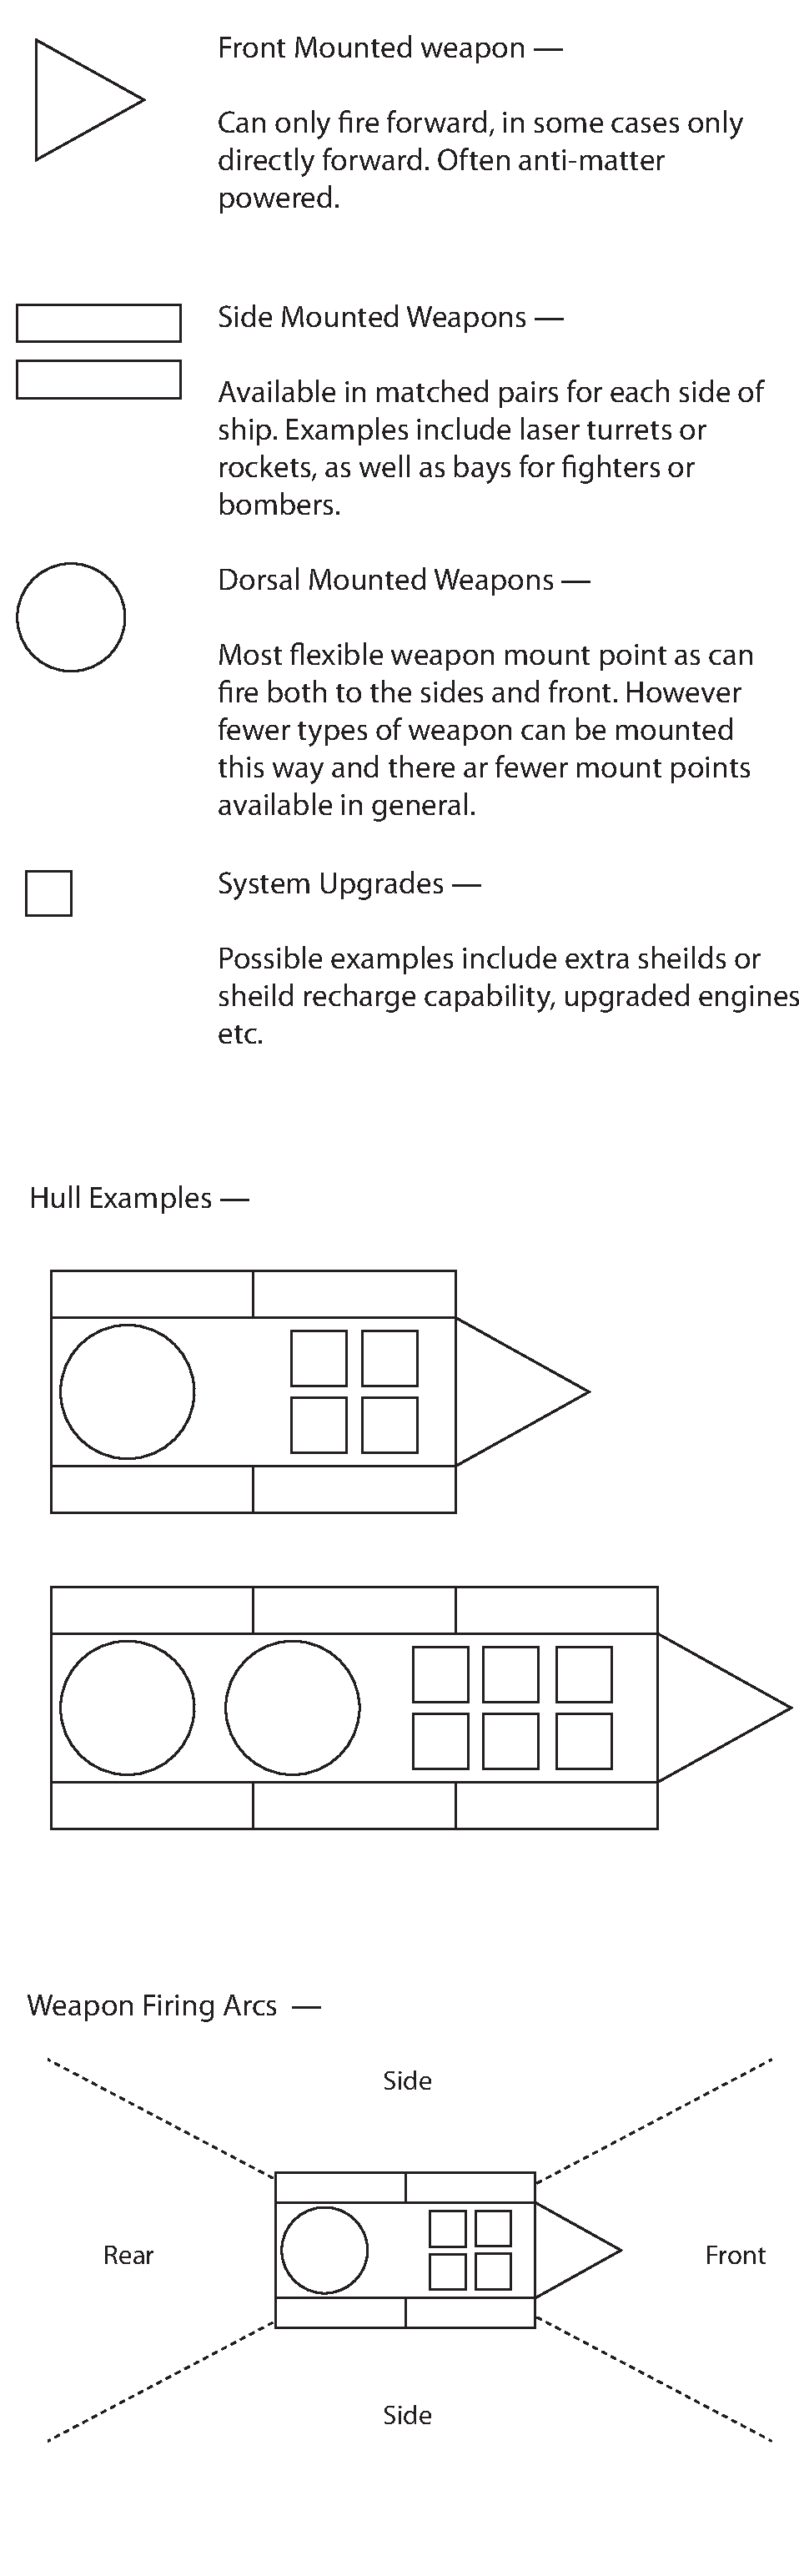
\includegraphics[width=6cm]{res/design/ship_design}
	\caption{Diagrams showing basic conception of ship customisation and weapon configurations. }
	\label{fig:ship_design}
\end{marginfigure}

\begin{description}

	\item[Multiplayer] As a multiplayer game, two players must be able to participate in a battle against each other.
	These players will be on different computers on the same network. This is a more attainable requirement than supporting play over the internet, as latency and packet loss issues will be less intrusive.

	\item[Fleets] Each player will control a fleet of ships. Ships have two health stats: hull and shields. Once hull health has been reduced to zero then the ship is destroyed. However, functioning shields prevent hull damage. It is intended that shields be relatively fast to recharge but hull damage is slow and expensive to repair.

	\item[Ship Customisation] The ships that make up a player's fleet will each have a number of pluggable slots. Prior to a game each player will be able to customise the ships in their fleet by filling these slots with different pieces of equipment. There will be two types of slot: system slots and weapons slots, the latter also split into the areas on the ship it can be installed on. System slots allow for extra internal systems to be added to the ship, for example extra shields or long range scanners. Weapons slots allow the player to choose which types of weapons their ships will use; however, a fleet budget will prevent a user from using the best weapons on every ship. See figure \ref{fig:ship_design}.

	\item[Resource System] Three resources exist within the game: fuel, metal, and anti-matter. These resources are only used by the ships. Fuel maintains a ship's shields, without a shield any damage will be done to the ship's hull. Metal is used to slowly repair a ship's hull after it has been damaged. Anti-matter is a rare resource that is used by the more powerful weapons available.

	Planets generate a constant supply of resources, so players can gain extra resources via planetary capture. The resources generated by the planets owned by a player feed into that player's global stockpile. Individual ships then draw resources from this stockpile.

	% Do ships get resources from the stockpile automatically, or do they have to visit planets?

	\item[Planetary Capture] Planet ownership is the only method of generating resources. Planets can only belong to
	one player at a time at most. To capture a planet, a player must have their ships in control
	of the planet for a certain period of time. If the planet belongs to the enemy then it will
	take twice as long for it to be captured than an unoccupied planet.

	% \item[Tactical Zoom]

\begin{figure*}[t!]
	\includegraphics[width=16cm]{res/design/mockup1}
	\caption[][1em]{Initial mockup of a screen during gameplay, showing a planet, navigation lines, selected ships, minimap, and reports from other ships.}
	\label{fig:mockup1}
\end{figure*}

	\item[Fog of War] Players must not be able to see the state of the entire map unless they control it all. There
	will be three levels to the fog of war: unknown, visited, and visible. Any locations on the map
	that a player's ships have not visited will be `unknown' and the player will not be able to see
	anything that is at that location. Any locations that have been explored at least once will be
	`visited'; the player will be able to see the general layout of the area, but not any details
	such as enemy ships. Finally, any locations covered by planets or ships owned by the player will
	be `visible' and all aspects of the map in the area will be revealed.
	
	\item[AI] A sophisticated artificial intelligence system will be an important component in the game.
	Each player's fleet will be controlled through an AI system. It will use a planning algorithm
	that takes a high level objective given by the player and generates a series of steps to
	achieve that objective. The AI must control the individual ships that make up the fleet; it
	is up to the human player to decide on the overall strategy of the fleet.

	A successful AI system must receive orders and quickly convert them into a sensible plan which it performs and reviews autonomously. If an impossible goal is set, or an existing goal is
	invalidated by changes to the world, then the AI must detect this and act accordingly.

	% Basic AI elements, e.g. pathfinding

	\item[Campaign] A campaign mode will be available which consists of a fixed number of battles between the two players.
	The final battle will be the `showdown' that determines the overall winner. The victor of each of
	the earlier battles will be granted bonuses toward the final battle, giving them an advantage against
	their opponent.

	Between every battle each player will have an opportunity to perform minor customisations on
	the ships in their fleet.

	\item[Operating System Requirements] The game must be playable on recent versions of Mac OS X and Linux. The nature of the libraries that are likely to be used for development make it possible that also supporting Windows will be relatively easy, but this is not guaranteed and no commitment on it is being made at this stage.

% \item[Gameplay]
% mention ship destruction and resources that drained during battle, not loss of ships

\end{description}

\subsection{Non-Functional Requirements}

\begin{description}

	\item[Fun] One of the most important requirements is that the game should be fun to play. Players should enjoy the game and want to play it multiple times.

	\item[Short game sessions] An individual battle should not last too long. If a game is likely to take a number of hours it is a barrier to entry for players as they must schedule large amounts of their time if they are to play at all. The aim should be for an individual battle to last between 20 and 35 minutes. Tournaments or campaigns are possible optional features that could extend this to provide inbuilt support for longer playing sessions.
	
	\item[Approachable]  An end user should be able to play a networked game with minimal configuration (no more configuration required than a typical installation and networking configuration).

	\item[Reliable] Both the client and server should be stable programs that are not prone to crashing. If either were to crash regularly then it would ruin the experience and cause people to stop playing the game.

	The networking component should also be reliable. Minor network disruption should not cause a huge loss in communication between the clients and server.

	\item[Secure] Although the game server will initially be intended for LAN usage it is important that it should not cause a computer running it on the Internet to be exploitable. It should not be vulnerable to attacks such as denial of service, which would stop the machine from performing any other tasks whilst under attack, or remote code execution, which could allow an attacker to take control of the target machine. 
	
	Furthermore, the game system should should not be vulnerable to cheating by modification of the client code, packet injection attacks, or other similar methods of gaining an unfair advantage. 

	% Macromanagement?

\end{description}


